%%%%%%%%%%%%%%%%%%%%%%%%%%%%%%%%%%%%%%%%%%%%%%%%%%%%%%%%%%%%%%%%%%%%
\section{Anode Plane Assembly (APA) Overview}
\label{sec:fdsp-apa-intro}

The \dwords{apa}, or wire planes, are the \dword{dune} \dword{sp} module elements used to sense, through both signal induction and direct collection, the ionization electrons created when charged particles traverse the \dword{lar} volume inside the \dword{spmod}.   All elements of the \dword{dune} physics program depend on a high performing system of \dword{apa}s and their associated readout \dword{ce}.  

Volume~\volnumberphysics{} of this \dword{tdr}, \voltitlephysics, % The Physics,  \dword{tdr}, Vol.~2, 
describes the simulations that rigorously establish the requirements for achieving the needed performance.  Here we summarize some of the \dword{apa} capabilities required for the key elements of neutrino \dword{cpv} and associated long-baseline oscillation physics, \dword{ndk}, and intra-galactic \dword{snb} searches.  As a multipurpose detector accessing physics from MeV to multi-GeV scales, the \dword{dune} \dword{lartpc} cannot be optimized for a narrow range of interaction signatures in the manner of noble liquid \dwords{tpc} dedicated to direct \dword{dm} or neutrino-less double beta decay searches.  The \dword{apa}s must collect ionization charge in a way that preserves the spatial and energy profiles of ionization events that range from few hundred keV point-like depositions (from low energy electrons and neutrons created in \dword{snb} neutrino interactions) to the double-kinked $K\rightarrow\mu\rightarrow{e}$ decay chain with its combination of highly- and minimum-ionizing particles (HIPs and MIPs) that is a key signature in proton decay searches.  The \dword{apa}s must record enough hits on tracks within a few cm of a neutrino interaction vertex to differentiate the 1 \dword{mip} $dE/dx$ signature of a $\nu_e$-induced electron from the 2 \dword{mip} signature of a $\nu$ neutral current photon conversion to enable the $\nu_\mu-\nu_e$ separation demanded for \dword{cpv} physics; and they must provide the pattern recognition and calorimetry for multi-GeV neutrino interaction products  spread over cubic meters of the detector needed for the precision neutrino energy estimates that allow separation of \dword{cpv} effects from those related to matter effects. 
 
Anode planes in the \dword{apa} must be well-shielded from possible high voltage breakdown events in the \dword{detmodule}.  The \dword{apa} wire spacing and orientations must maximize pattern recognition capabilities and \dword{s/n} in a cost-effective manner.  The \dword{apa} wires must maintain their positions to a level that is small compared to the wire spacing so that energy estimators based on range and multiple Coulomb scattering remain reliable over two decades of operation.  The wires must hold their tension, lest microphonic oscillations develop that degrade \dword{s/n} or anode plane field distortions arise that inhibit the transmission of drifting electrons through the induction planes to the collection plane.  Any wire break would destroy \dwords{fv}, so the \dword{apa} design must both minimize the possibility of this occurrence and contain the extent of any damage that would ensue should it happen.  An \dword{apa} implementation that meets all these goals follows in the remainder of this chapter, along with a summary of significant validations achieved through dedicated simulations and \dword{pdsp} construction and operations.


\begin{dunefigure}[A \nominalmodsize DUNE far detector SP module]{fig:DUNESchematic1ch1}
{A \nominalmodsize \dword{dune} \dword{fd} \dword{spmod}, showing the alternating \sptpclen{} long (into the page), \tpcheight{} high anode (A) and cathode (C) planes, as well as the \dfirst{fc} that surrounds the drift regions between the anode and cathode planes. On the right-hand cathode plane, the foremost portion of the \dword{fc} is shown in its undeployed (folded) state.}
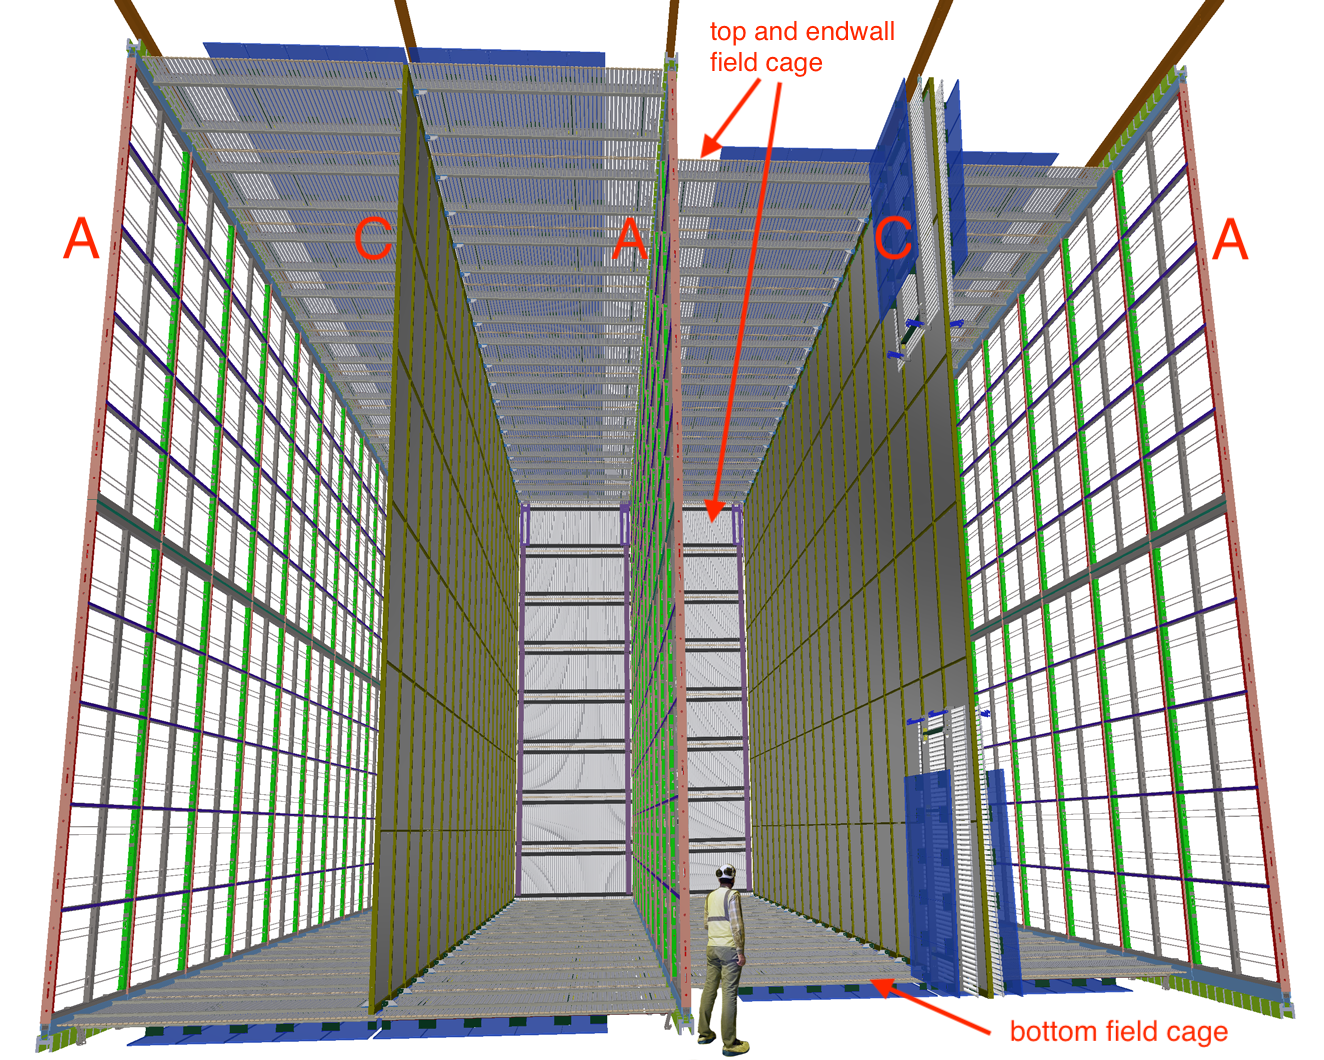
\includegraphics[width=0.65\textwidth]{DUNESchematic.png}
\end{dunefigure}
% anne replaced because it shows scale

To facilitate fabrication and installation underground, the anode design is modular, with \dword{apa}s tiled together to form the readout system for a \nominalmodsize \dword{detmodule}. A single \dword{apa} is \SI{6}{m} high by \SI{2.3}{m} wide, but two of them are connected vertically, and twenty-five of these vertical stacks are linked together to define a \tpcheight %\SI{12}{m} 
tall by \sptpclen %\SI{58}{m} 
long mostly-active readout plane.  As described below, the planes are active on both sides, so three such wire readout arrays (each one \tpcheight$\,\times\,$\sptpclen) %(each one \num{12}$\times$\SI{58}{m^2}) 
are interleaved with two \dword{hv} surfaces to define four \spmaxdrift %\SI{3.6}{m} 
wide drift regions inside each \dword{spmod}, as Figure~\ref{fig:DUNESchematic1ch1} shows in the detector schematic views. Each \dword{sp} \nominalmodsize module, therefore, will contain 150 \dword{apa}s.

Each \dword{apa} frame is covered by more than \num{2500} sense wires laid in three planes  oriented at angles to each other: a vertical collection plane, $X$, and two induction planes at \apainducwireangle to the vertical, $U$ and $V$. Having three planes allows multi-dimensional reconstruction of particle tracks even when the particle propagates parallel to one of the wire plane directions.  An additional \num{960} wires that are not read out make up an outer shielding plane, $G$, to improve signal shapes on the $U$ induction channels.  The angled wires are wrapped around the frame from one side to the other, allowing all channels to be read out from one end of the \dword{apa} only (the top or bottom), thereby minimizing the dead regions between neighboring \dword{apa}s. Signals induced or collected on the wires are transferred through soldered connections to wire termination boards mounted at the end of the \dword{apa} frame that in turn connect to \dword{fe} readout \dword{ce} sitting in the \dword{lar}.  Figures~\ref{fig:tpc_apa1} and \ref{fig:sp-apa-head-xsec} illustrate the layout of the wires on an \dword{apa}, showing how they wrap around the frame and terminate on wire boards at the head end where readout \dword{ce} are mounted.

The \dword{apa}s are a critical interface point between the various detector subsystems within the \dword{spmod}.  As already mentioned, the \dword{tpc} readout \dword{ce} mount directly to the \dword{apa} frames.  The \dwords{pd} for detecting scintillation light produced in the \dword{lar} are also housed inside the frames, sandwiched between the wires on the two sides, requiring careful coordination in frame design as well as requiring transparency for the \dword{apa} structures.  In addition, the electric \dfirst{fc} panels connect directly to the edges of the \dword{apa} frames.  Finally, the \dword{apa}s must support routing cables for both the \dword{tpc} electronics and the \dword{pd} systems. All these considerations are important to the design, fabrication, and installation planning of the \dword{apa}s.

\begin{dunefigure}[Illustration of the APA wire layout]{fig:tpc_apa1}
{Illustration of the \dword{dune} \dword{apa} wire wrapping scheme showing small portions of the wires from the three signal planes ($U,V,X$). The fourth wire plane ($G$) above these three, and parallel to $X$, is present to improve the pulse shape on the $U$ plane signals. The \dword{tpc} electronics boxes, shown in blue on the right, mount directly to the frame and process signals from both the collection and induction channels. The \dword{apa} is shown turned on its side in a horizontal orientation.} 
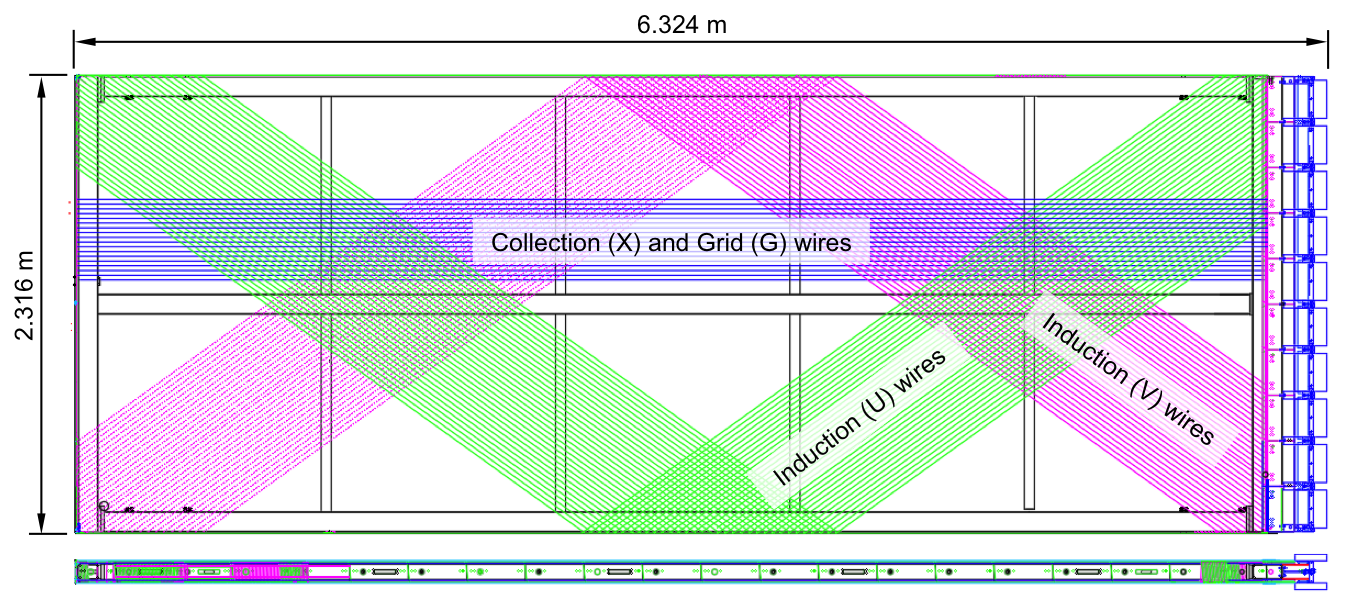
\includegraphics[width=\textwidth,trim = 0mm 10mm 0mm 0mm,clip]{sp-apa-drawing-wire-configuration.png} 
\end{dunefigure} 

\begin{dunefigure}[Cross section view of the head end and wire layers of an APA]{fig:sp-apa-head-xsec}
{Cross section view of an \dword{apa} frame near the head end showing the layers of wires ($G,U,V,X$) on both sides of the frame that terminate on wire boards, which connect to \dword{tpc} readout \dword{ce} through a capacitor-resistor chain on the \dword{cr} boards and a connector adapter board.} 
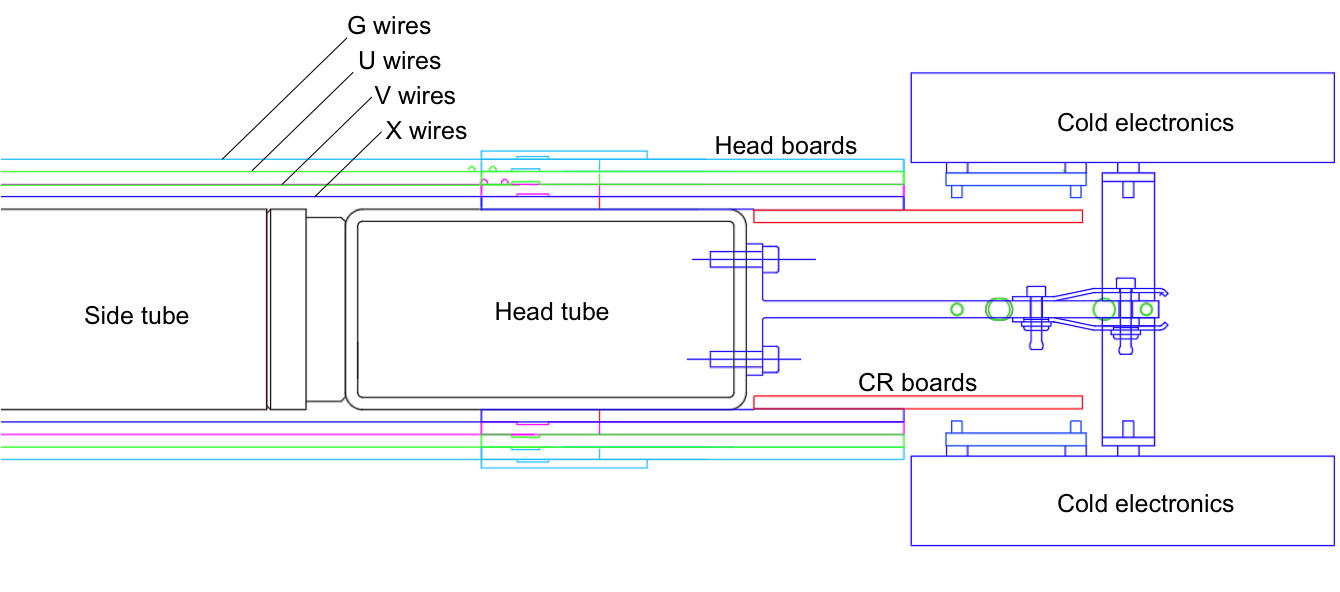
\includegraphics[width=1\textwidth]{sp-apa-drawing-cross-section.png} 
\end{dunefigure} 


The \dword{apa} consortium %within the \dword{dune} collaboration 
oversees the design, construction, testing, and installation of the \dword{apa}s. Several \dword{apa} production sites will be set up in both the US and the UK with each nation producing  half of the \dword{apa}s needed for the %DUNE 
\dwords{spmod}.  Production site setup is anticipated to begin in 2020, with \dword{apa} fabrication for the first \nominalmodsize \dword{spmod} running from 2021--2023.  

The Physical Sciences Laboratory (PSL) at the University of Wisconsin and the Daresbury Laboratory in the UK have recently produced full-scale \dword{apa}s for the \dword{pdsp} project at \dword{cern}. Figure~\ref{fig:apa-photo} shows a completed \dword{apa} produced at PSL just before shipment to \dword{cern}. % for use in \dword{pdsp}. 
This effort has greatly informed the design and production planning for the \dword{dune} \dwords{detmodule}, and \dword{pdsp} running has provided valuable validation for many fundamental aspects of the  \dword{apa} design. 

The remainder of this chapter is laid out as follows.  In Section~\ref{sec:fdsp-apa-design}, we present an overview of the design of the \dword{apa}s, focusing on the key design parameters and their connection to the physics requirements of \dword{dune}.  In Section~\ref{sec:fdsp-apa-qa}, we discuss quality assurance for the design with an emphasis on lessons learned from \dword{pdsp} construction and operations and a summary of remaining prototyping efforts being planned before the start of production next year. Section~\ref{sec:fdsp-apa-intfc} summarizes three important interfaces to the \dword{apa}s: \dword{tpc} cold electronics (\dword{ce}), photon detectors (\dword{pd}), and the cable routing for both systems.  In Section~\ref{sec:fdsp-apa-prod}, we detail the production plan for fabricating the large number of \dword{apa}s needed for the experiment including a description of the main construction sites being developed in the US and UK by the \dword{apa} consortium.  Section~\ref{sec:fdsp-apa-transport} describes some requirements for handling the large and delicate \dword{apa}s throughout construction and presents the design for a custom transport system for delivery to the far detector site for installation. Section~\ref{sec:fdsp-apa-safety} reviews the safety considerations for \dword{apa} construction and handling. Finally,  Section~\ref{sec:fdsp-apa-org} summarizes the organization of the \dword{apa} consortium that is responsible for building the \dword{apa}s and provides the high-level cost, schedule, and risk summary tables for the project. 

\begin{dunefigure}[A completed APA for \dshort{pdsp}]{fig:apa-photo}
{Completed \dshort{pdsp} \dshort{apa} ready for shipment to \dword{cern}.}
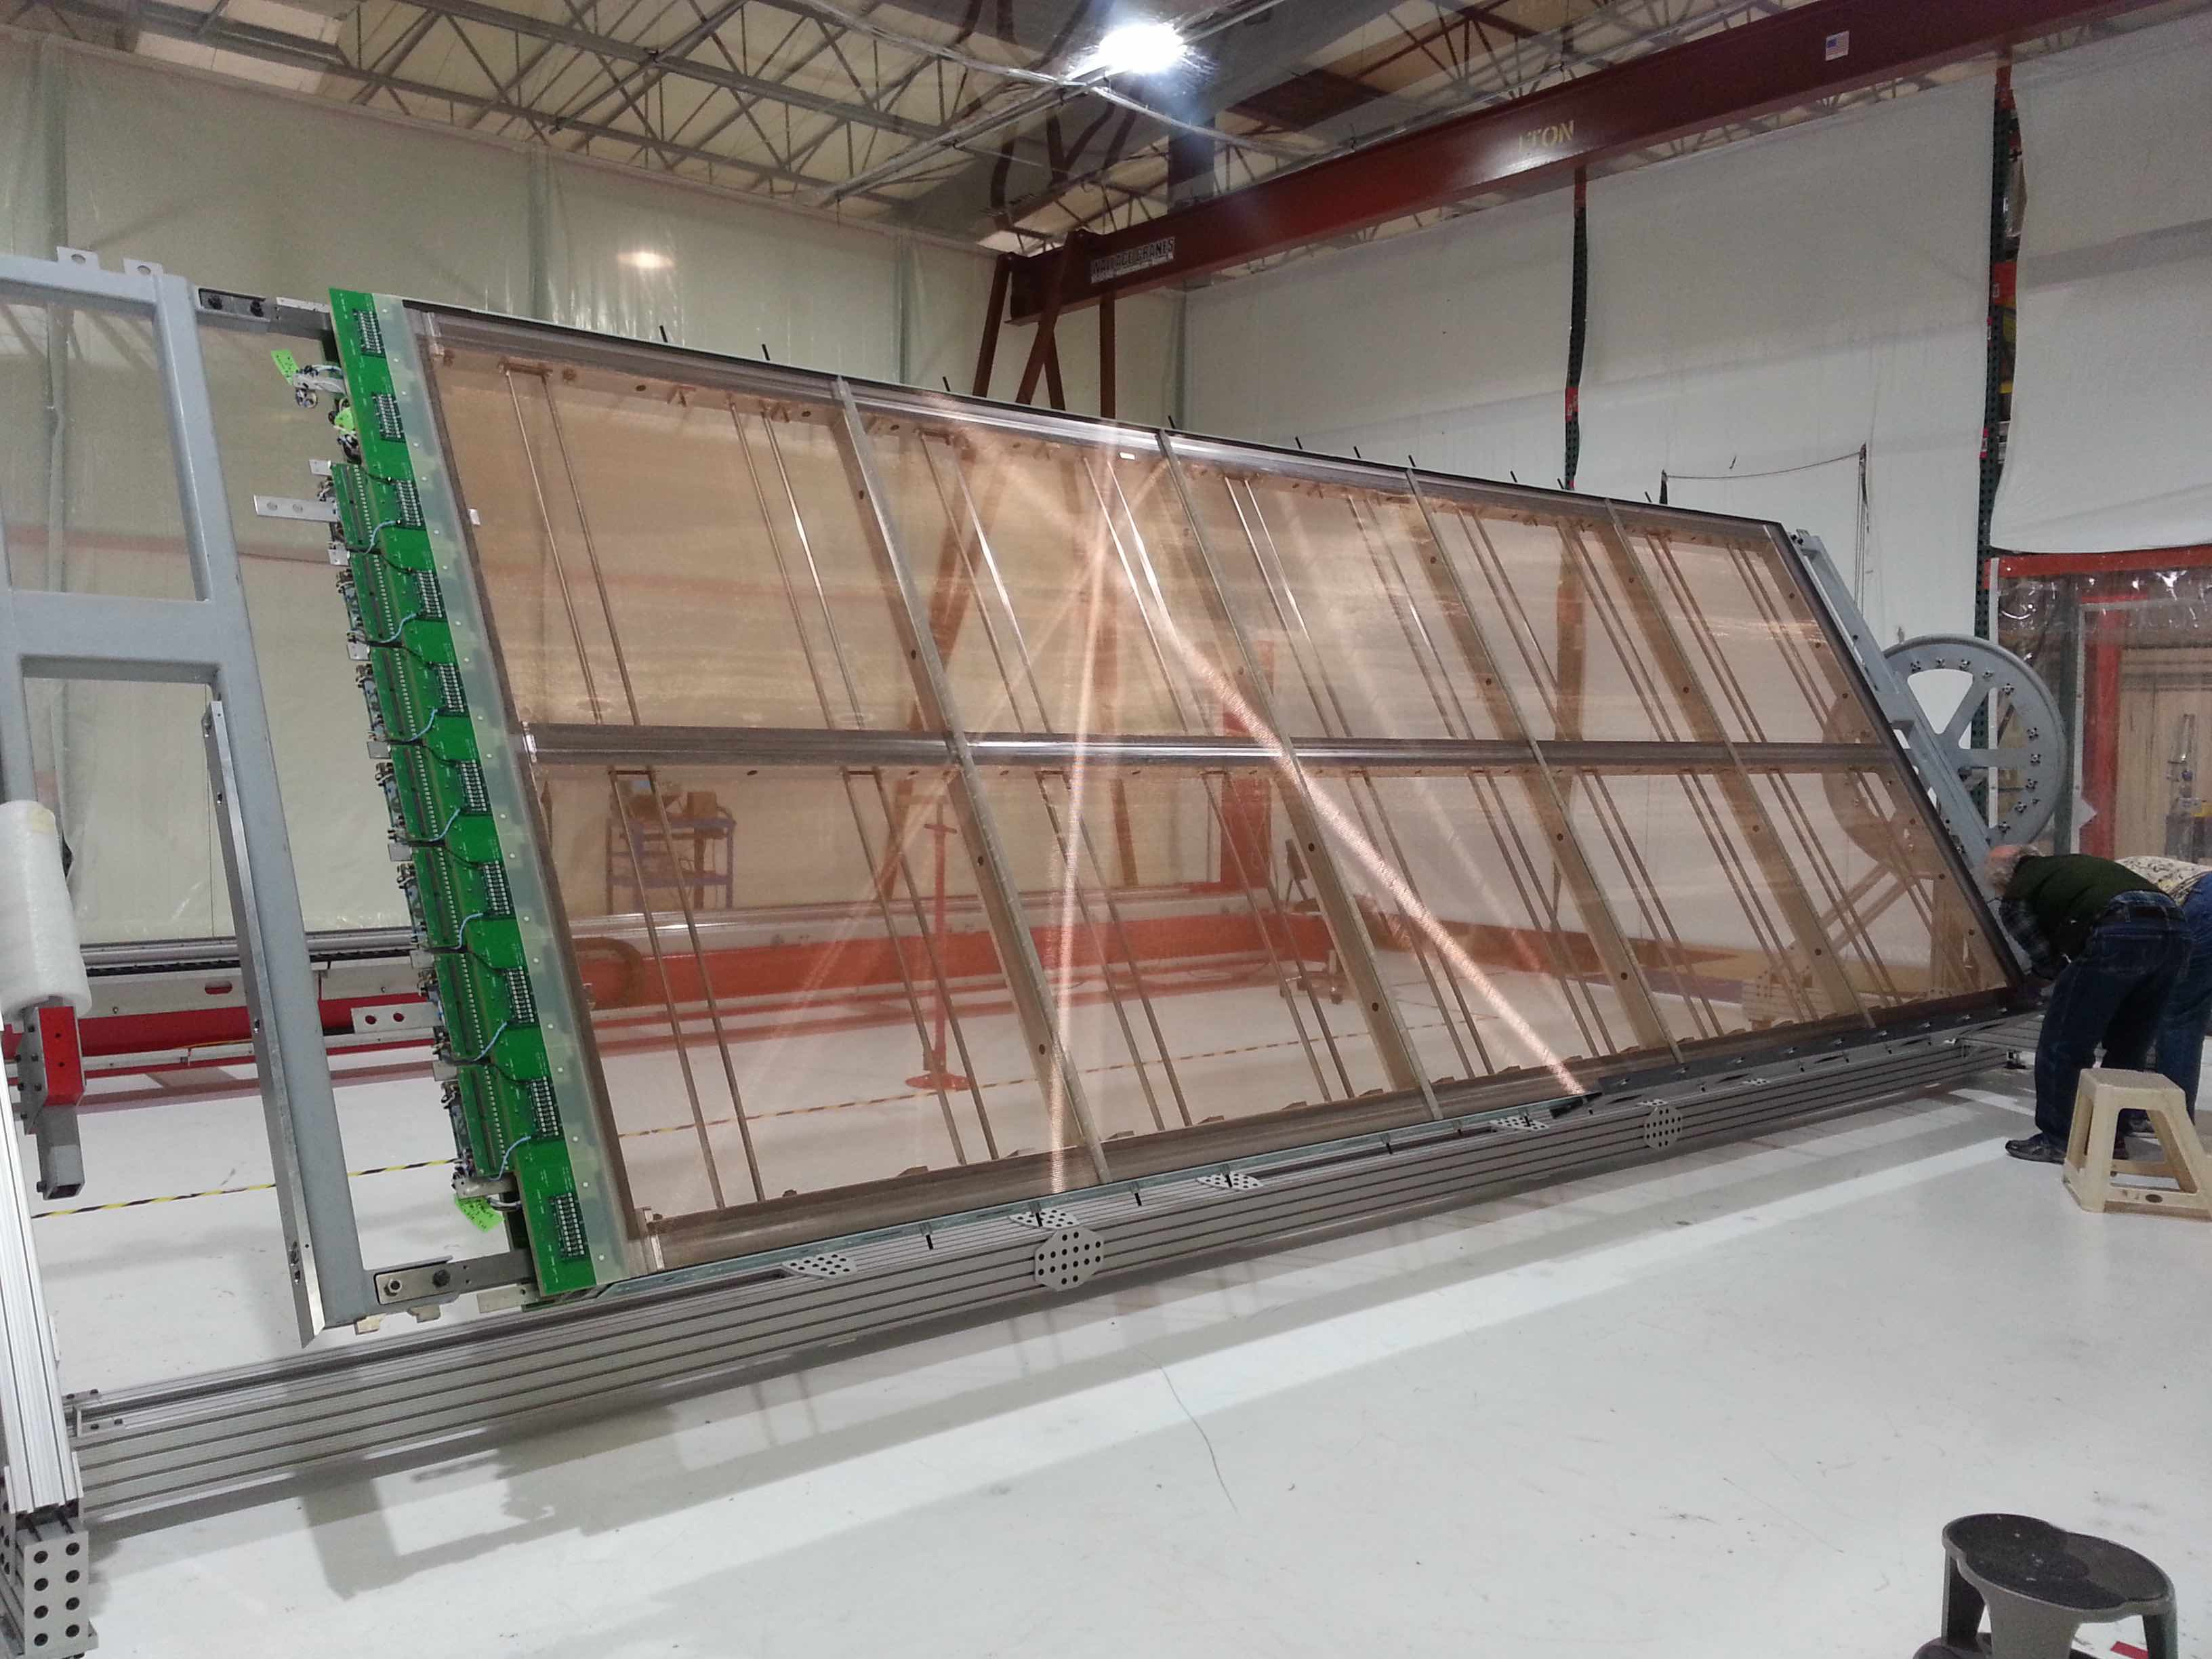
\includegraphics[width=1.0\textwidth,trim=20mm 80mm 0mm 60mm,clip]{sp-apa-photo-complete.jpg}
\end{dunefigure}
